% =============================================================================
% backup.tex — Q&A backup slides (\appendix, δεν μετριούνται)
% =============================================================================

\begin{frame}{Σλαίδς Q\&A}
  \centering\Large
  \vfill
  \textbf{Αντίγραφα Q\&A} \\ \vspace{0.5em}
  \normalsizeΠαρακάτω \en{slides} για ερωτήσεις
  \vfill
\end{frame}

% --- B1: Constant-time (backup only per user decision) ---
\begin{frame}{\en{Constant-time}: \en{Zkt} επαληθεύει \en{Tier~1/2 scalar/RVV} για \en{dudect}}
  \begin{columns}[T]
    \begin{column}{0.55\textwidth}
      \begin{itemize}
        \item \defterm{\en{Zkt}}: επεκτατική επίπεδο \en{RISC-V} για σταθερή \en{latency} εντολών (\en{integer/bitmanip})
        \item \en{clmul}: εντός \en{Zkt} (\en{constant-time guaranteed} από \en{ISA spec})
        \item \en{Tier~1/2}: δοκιμασμένα με \en{dudect} (δισταστικός ελεγχός \en{t-test})
              $\to$ \pos{κανένα λείψιμο σήμα \en{timing} διακύμανσης}
        \item \en{Tier~3} (\vclmul): \con{δεν ερευνήθηκε ακόμα} — \en{Zkt} καθορισμός εκκρεμής
        \item \en{Reed-Muller/Solomon} \Decaps: \en{branchless} υλοποίηση
      \end{itemize}
    \end{column}
    \begin{column}{0.43\textwidth}
      \begin{block}{\en{Zkt} καλυπτόμενες εντολές}
        \begin{itemize}\footnotesize
          \item \en{Integer ALU, shifts, loads, stores}
          \item \en{Zba/Zbs/Zbb}: \en{bit-manip}
          \item \en{Zbc}: \clmul, \clmulh
          \item \en{Zbkb}: \en{crypto bitmanip}
          \item \con{\en{Zvbc vclmul}: \emph{not in Zkt spec}}
        \end{itemize}
      \end{block}
    \end{column}
  \end{columns}
\end{frame}

% --- B2: ISA ablation (Zba/Zbs waterfall) ---
\begin{frame}{\en{ISA Ablation}: συνεισφορά κάθε επέκτασης \en{(Tier~1)}}
  \begin{columns}[T]
    \begin{column}{0.50\textwidth}
      \begin{itemize}
        \item \textbf{\en{Waterfall}}: αφαίρεση μίας-μίας επέκτασης από \en{Tier~1}
        \item Σημαντική συνεισφορά: \Zbc (\clmul) κυρίαρχεί
        \item \Zbb (για \en{Keccak rori}): \emph{επιπλέον} \speedup στον συνολικό \en{KEM}
        \item \Zba/\Zbb: \en{address/bitmask} αριθμητικές εντολές — μικρός αριθμός αποθηκευμένων εντολών
        \item \en{Baseline}: \en{RV64G} μόνο (\emph{χωρίς} επεκτάσεις) — αφετηρία του \en{schoolbook}
      \end{itemize}
    \end{column}
    \begin{column}{0.48\textwidth}
      \begin{block}{\en{Tier~1} συνεισφορά κατά επέκταση (\en{HQC-128 \instret})}
        \footnotesize
        \begin{tabular}{@{}lr@{}}
          \toprule
          \en{Config} & \speedup{} πολ\textperiodcenteredπολ. \\
          \midrule
          \en{RV64G} (βάση) & $1.0\times$ \\
          + \Zba & $1.0\times$ \\
          + \Zbb & $1.1\times$ \\
          + \Zbc \clmul & \HL{$101\times$} \\
          \bottomrule
        \end{tabular}\\
        \vspace{0.3em}\scriptsize \Zbc είναι \emph{by far} η κυρίαρχη συνεισφορά
      \end{block}
    \end{column}
  \end{columns}
\end{frame}

% --- B3: VLEN scaling ---
\begin{frame}{\VLEN επέκταση (\en{Tier~2/3})}
  \begin{columns}[T]
    \begin{column}{0.54\textwidth}
      \centering
      \resizebox{\columnwidth}{!}{%
        % Line chart: Security level (x) vs Decaps instret (y) per variant
% Shows scaling behavior — log-log scale reveals power-law exponents
\tikzsetnextfilename{ch8-results-scaling-security-line}
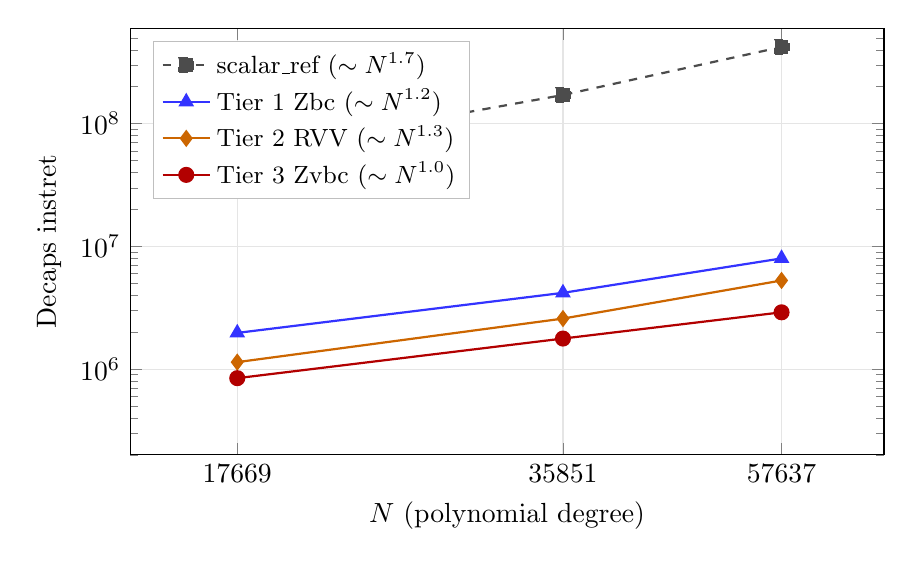
\begin{tikzpicture}
\begin{axis}[
  width=0.92\linewidth,
  height=7cm,
  xlabel={$N$ (polynomial degree)},
  ylabel={Decaps instret},
  xmode=log,
  ymode=log,
  log basis x=2,
  xtick={17669, 35851, 57637},
  xticklabels={\num{17669}, \num{35851}, \num{57637}},
  xmin=14000, xmax=72000,
  ymin=2e5, ymax=6e8,
  legend style={
    at={(0.03,0.97)},
    anchor=north west,
    font=\small,
    cells={anchor=west},
    draw=gray!50,
  },
  grid=major,
  grid style={gray!20},
  every axis plot/.append style={thick, mark size=2.5pt},
]

% scalar_ref: schoolbook O(N^2)
\addplot[color=black!70, mark=square*, dashed]
  coordinates {(17669, 56937074) (35851, 171349089) (57637, 421860950)};
\addlegendentry{scalar\_ref ($\sim N^{1.7}$)}

% Tier 1: Karatsuba Zbc
\addplot[color=blue!80, mark=triangle*]
  coordinates {(17669, 1972347) (35851, 4181542) (57637, 7980756)};
\addlegendentry{Tier~1 Zbc ($\sim N^{1.2}$)}

% Tier 2: Karatsuba RVV
\addplot[color=orange!80!black, mark=diamond*]
  coordinates {(17669, 1139356) (35851, 2579762) (57637, 5274100)};
\addlegendentry{Tier~2 RVV ($\sim N^{1.3}$)}

% Tier 3: Karatsuba Zvbc
\addplot[color=red!70!black, mark=*]
  coordinates {(17669, 843459) (35851, 1773770) (57637, 2902352)};
\addlegendentry{Tier~3 Zvbc ($\sim N^{1.0}$)}

\end{axis}
\end{tikzpicture}
%
      }
    \end{column}
    \begin{column}{0.44\textwidth}
      \begin{itemize}
        \item \VLEN καλύπτει {128, 256, 512, 1024}
        \item \en{BPI-F3 / SpacemiT K1}: \VLEN~=~256
        \item \pos{Υψηλότερο \VLEN}: απευθείας επιτάχυνση \polymul
        \item \en{HQC-256} λαμβάνει μεγαλύτερη απόδοση από \VLEN scaling
        \item \en{Keccak} ανεξάρτητο από \VLEN
      \end{itemize}
    \end{column}
  \end{columns}
\end{frame}

% --- B4: Detailed microbenchmark instret ---
\begin{frame}{Αναλυτικό \en{microbenchmark}: \instret ανά \en{tier} \& επίπεδο ασφάλειας}
  \centering
  \resizebox{0.88\textwidth}{!}{%
    % Grouped bar chart: micro-benchmark instret comparison (HQC-128)
% Shows Reference vs Tier 1/2/3 for each kernel
\tikzsetnextfilename{ch8-results-microbench-bar-chart}
\begin{tikzpicture}
\begin{axis}[
    ybar,
    bar width=10pt,
    width=0.95\textwidth,
    height=7cm,
    ymode=log,
    log origin=infty,
    ylabel={Δυναμικές εντολές (\instret)},
    symbolic x coords={Polymul, Keccak, Decode},
    xtick=data,
    x tick label style={font=\small},
    ymin=10000,
    ymax=100000000,
    legend style={
      at={(0.5,1.03)},
      anchor=south,
      legend columns=3,
      font=\footnotesize,
      /tikz/every even column/.append style={column sep=8pt}
    },
    nodes near coords style={font=\tiny, rotate=90, anchor=west},
    enlarge x limits=0.25,
    grid=major,
    ymajorgrids=true,
    xmajorgrids=false,
]

% Reference (scalar baseline)
\addplot[fill=gray!60, draw=gray!80] coordinates {
    (Polymul, 18504302)
    (Keccak, 758580)
    (Decode, 1052692)
};

% Tier 1 (scalar_zb polymul / opt keccak / scalar-zb decode)
\addplot[fill=blue!50, draw=blue!70] coordinates {
    (Polymul, 182726)
    (Keccak, 554900)
    (Decode, 604218)
};

% Tier 2 (vector_rvv polymul / opt keccak / rvv decode)
\addplot[fill=orange!60, draw=orange!80] coordinates {
    (Polymul, 148479)
    (Keccak, 554900)
    (Decode, 134737)
};

% Tier 3 (vector_zvk polymul / zvbb keccak / zvbc decode)
\addplot[fill=green!50, draw=green!70] coordinates {
    (Polymul, 70070)
    (Keccak, 554900)
    (Decode, 73769)
};

\legend{Reference, Tier~1 (\Zbc), Tier~2 (RVV), Tier~3 (\Zvbc/\Zvbb)}

\end{axis}
\end{tikzpicture}
%
  }
\end{frame}

% --- B5: Compiler comparison ---
\begin{frame}{\en{GCC vs Clang}: αμελητέα διαφορά για \en{Tier~1}}
  \begin{itemize}
    \item \en{GCC~14} και \en{Clang~18} βαθμολογήθηκαν με \en{-O3 -LTO}
    \item \pos{Αμελητέα διαφορά} \en{Tier~1}: αμφότεροι εκφέρουν \clmul σωστά
    \item \en{Tier~2}: \en{GCC} ελαφρώς υπερέχει στη διανυσματική ανασύνθεση
    \item \en{Tier~3}: αριθμητικά εως +2\% διαφορά λόγω \en{inline} στρατηγικής
    \item \emph{Επιλογή}: \en{GCC~14} αρχείο \en{benchmark}; αποτελέσματα ανεξάρτητα \en{compiler}
  \end{itemize}
\end{frame}

% --- B6: Karatsuba tree pseudocode ---
\begin{frame}[fragile]{\en{Karatsuba} δέντρο στο $\GFpoly$ σε \en{C} (\en{Tier~1} εσωτερική δομή)}
  \begin{columns}[T]
    \begin{column}{0.50\textwidth}
\begin{lstlisting}[language=C,caption={}]
// Tier1: statically generated Karatsuba
// in GF(2)[x]; no runtime branches.
// a_hi, a_lo: 64-bit word halves of a
// clmul64 -> carry-less mul (Zbc clmul)
static void karatsuba_gf2(
    uint64_t a_hi, uint64_t a_lo,
    uint64_t b_hi, uint64_t b_lo,
    uint64_t *res) {
  uint64_t lo = clmul64(a_lo, b_lo);
  uint64_t hi = clmul64(a_hi, b_hi);
  uint64_t mid = clmul64(
    a_lo ^ a_hi, b_lo ^ b_hi);
  res[0] ^= lo;
  res[1] ^= lo >> 63 ^ hi ^ mid;
  res[2] ^= hi >> 1;
}
\end{lstlisting}
    \end{column}
    \begin{column}{0.48\textwidth}
      \begin{itemize}\small
        \item 3 \clmul \en{vs.} 4 (βελτίωση 25\%)
        \item Αναδρομή στο \en{compile time}: \en{O(1)} μόνοι στόιβα
        \item \en{Assign-on-first-write}: αποφεύγεται αρχικοποίηση πίνακα
        \item \en{Full HQC-128 polymul}: $\approx\num{276}$ \clmul
      \end{itemize}
    \end{column}
  \end{columns}
\end{frame}
